\section{Evaluation}

\subsection{Detailed evaluation of examples}

Let us consider the following example:
$\alpha_1 = \{x_1 - x_2 \geq -4, -x_2 - x_3 \geq 5, 
  x_2 + x_6 \geq 4, x_2 + x_5 \geq -3\}; 
\beta_1 = \{-x_1 + x_3 \geq -2, -x_4 - x_6 \geq 0, -x_5 + x_4 \geq 0\}$. 
Our implementation produces the following trace:

\verbatiminput{../../Software/Cpp/OctagonsInterpolant/tests/traces/example1.txt}

The Z3 SMT solver provides mechanisms to modified the arithmetic engine 
and several plugins to specialize algorithm for specific theories. It contains a
proper specialization to work with Utvpi queries for satisfiability checking. However, 
       the interpolation APIs do not include mechanisms to specialize the 
       interpolation algorithm for Utvpi formulas. Thus, the interpolant obtained by Z3 
       for the above problem is : 
       (and ($\leq$ 9 (+ (* (- 1) x3) (* 2 x6) x1)) ($\leq$ (- 5) (+ (* (- 1) x3) (* 2 x5) x1))).
       We can notice by the coefficients in the result that the interpolant is not
       a Utvpi formula, thus Z3 must have reduced the problem to linear integer arithmetic.

  The result obtained by Mathsat is 
(and ($\leq$ (- 5) (+ x1 (+ (* (- 1) x3) (* 2 x5)))) ($\leq$ 9 (+ x1 (+ (* (- 1) x3) (* 2 x6))))) 
  which is the same as Z3 modulo the commutativity of the
  additions in the expression. Despite this difference, the following query 
  to Z3 verifies that the interpolation produced by our implementation implies 
  the interpolation produced by the SMT solver above mentioned; at the same time,
  the interpolant produced by the SMT solver does not imply our interpolant.

  \verbatiminput{../../Software/Cpp/OctagonsInterpolant/verification/example1_strongest_inter_verification.smt2}

  For the next example, let us consider $\alpha_2 = \{
  -x_2 - x_1 + 3 \geq 0, 
  x_1 + x_3 + 1 \geq 0, 
  -x_3 - x_4 - 6 \geq 0, 
  x_5 + x_4 + 1 \geq 0 
  \}; \beta_2 = \{
  x_2 + x_3 + 3 \geq 0,
  x_6 - x_5 - 1 \geq 0,
  x_4 - x_6 + 4 \geq 0
  \}$. Our implementation produces the following trace:

\verbatiminput{../../Software/Cpp/OctagonsInterpolant/tests/traces/example2.txt}

The interpolant obtained by Z3 is 
 (and ($\leq$ (- 4) (+ x3 (* (- 1) x2))) ($\leq$ (+ x3 x4) (- 6)) ($\geq$ (+ x4 x5) (- 1))); 
 and the interpolant produced by Mathsat is ($\leq$ (+ x2 (+ x3 (+ x4 (* (- 1) x5)))) (- 7)).
 Using Z3, we were able to verify that: 
 \begin{itemize}
 \item the interpolantion obtained by our implementation
 is equivalent to the interpolant obtained by Z3. 
 \item the interpolant obtained by our implementation implies the interpolant
 obtained by Mathsat, but the converse does not hold.
 \end{itemize}

\verbatiminput{../../Software/Cpp/OctagonsInterpolant/verification/example2_strongest_inter_verification.smt2}

\subsection{Performance comparison with iZ3 and MathSat}\label{performance_oct}

This section discusses a parametrized problem 
in the UTVPI theory and compares the times required by
our implementation, iZ3, and Mathsat.

\begin{lemma} \label{performance_test_lemma_oct}
  Let $x_i$ for $1 \leq i \leq n$ where $n \in \mathbb{N}$ is fixed.
  The following conjunction of inequalities is unsatisfiable:
  \begin{equation*}\label{oct_problem}
    x_1 + x_2 \leq 1 
    \land \bigwedge_{i=2}^{n-1} (x_{i+1} - x_i \leq 1) 
    \land x_1 - x_n \leq 1
    \land x_1 > \ceil{n/2}
  \end{equation*}
\end{lemma}

\begin{proof}
  Using the first $n-1$ inequalities of the conjunction
  in \ref{oct_problem} we can conclude that $2x_1 \leq n$.
  The latter contradicts the last inequality $x_1 \cei{n/2}$.
\end{proof}

The interpolation pair for our performance test 
is $(x_1 + x_2 \leq 1 
    \land \bigwedge_{i=2}^{n-1} (x_{i+1} - x_i \leq 1) 
    \land x_1 - x_n \leq 1, x_1 > \ceil{n/2})$
for fixed $n \in \mathbb{N}$.
It is easy to see that the pair is inconsistent due to the lemma 
\ref{performance_test_lemma_oct}. 

By lemma \ref{performance_test_lemma_oct}
we can also see that the formula $x_1 \leq \ceil{n/2}$ is an 
interpolating formula for all fixed $n$ in this parametrized problem.
We designed this problem because it is easy to verify the 
correctness of output of the algorithms and to measure 
the time used by the algorithms for large values of $n$. 
We executed instances of this problem for values of $n$
in the range $\{1, \dots, 10000\}$ using the same setup 
used in the performance comparison for the parametrized 
problem discussed in \ref{performance_test_lemma}.
The follow graph shows similar results as 
in \ref{performance_test_lemma}.

\begin{figure}
  \centering
  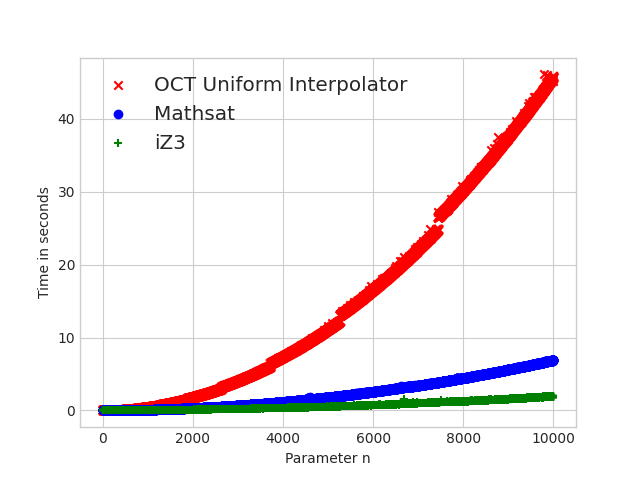
\includegraphics[scale=0.9]{figures/octi_performance_graph}
  \caption{Performance comparison graph of Oct interpolant generation
  algorithms for paramatrized problem from section \ref{performance_oct}} 
  \label{performance_graph_euf}
\end{figure}

We noticed a quadractic behaviour in the graph for the time 
required by all the algorithms. Indeed, the latter was
validated since a quadratic fitting has a smaller quadratic
error compared to a linear fitting in all the implementations
as show in the following table:

\begin{table}[h]
  \centering
  \begin{tabular}{ccc}
    \toprule
    {}                 & Error of linear fitting & Error of quadratic fitting \\
    \cmidrule{2-2} \cmidrule{3-3}                                             \\
    iZ3                & 3.2311742677852644e-25 & 1.269128969536517e-23       \\
    Mathsat            & 2.3207586060940883e-22 & 1.1983240884566356e-22      \\
    Our implementation & 2.9778502051908996e-21 & 1.455131710005814e-20       \\
    \bottomrule
  \end{tabular}
  \caption{Table of polynomial fitting errors of degrees 1, 2 for the
  Octagon experiments of section \ref{performance_oct}.}
\end{table}

%%% Local Variables:
%%% mode: latex
%%% TeX-master: "main"
%%% End:
